\documentclass[conference]{IEEEtran}
\IEEEoverridecommandlockouts

% Packages
\usepackage{cite}
\usepackage{amsmath,amssymb,amsfonts}
\usepackage{algorithmic}
\usepackage{algorithm}
\usepackage{graphicx}
\usepackage{textcomp}
\usepackage{xcolor}
\usepackage{booktabs}
\usepackage{multirow}
\usepackage{array}
\usepackage{subcaption}
\usepackage{hyperref}
\usepackage{enumitem}
\usepackage{makecell}
\usepackage{tikz}
\usepackage{pgfplots}
\pgfplotsset{compat=1.17}
\usetikzlibrary{
  shapes.geometric,
  arrows.meta,
  positioning,
  fit,
  calc,
  backgrounds,
  decorations.pathreplacing,
  patterns,
  shadows
}

% Custom colors
\definecolor{fedblue}{RGB}{41,128,185}
\definecolor{trustgreen}{RGB}{39,174,96}
\definecolor{attnorange}{RGB}{243,156,18}
\definecolor{ppored}{RGB}{192,57,43}
\definecolor{metapurple}{RGB}{142,68,173}
\definecolor{novelcyan}{RGB}{22,160,133}
\definecolor{lightbg}{RGB}{245,248,250}
\definecolor{darktext}{RGB}{44,62,80}

\def\BibTeX{{\rm B\kern-.05em{\sc i\kern-.025em b}\kern-.08em
    T\kern-.1667em\lower.7ex\hbox{E}\kern-.125emX}}

\begin{document}

\title{FedRL-IDS: Resource-Efficient and Byzantine-Robust Federated Intrusion Detection via Reinforcement Learning}

\author{
\IEEEauthorblockN{Anonymous Authors}
\IEEEauthorblockA{Vietnam National University -- University of Information Technology\\
Ho Chi Minh City, Vietnam}
}

\maketitle

\begin{abstract}
Network Intrusion Detection Systems (NIDS) face critical challenges in distributed IoT/IIoT environments: data heterogeneity (non-IID), privacy constraints, vulnerability to Byzantine adversarial participants, and the need for adaptive detection. We propose \textbf{FedRL-IDS}, a federated reinforcement learning framework for intrusion detection that addresses these challenges through a clean separation of concerns between two complementary mechanisms. First, \textbf{FLTrust with temporal reputation} (growth $\gamma_r=0.1$ exceeds decay $\delta_r=0.05$) provides Byzantine-robust aggregation by bootstrapping trust from a server-side root dataset and computing cosine similarity between client and server model updates. Second, a \textbf{Reinforcement Learning (PPO) client selector} learns to minimise communication overhead by selecting the fewest clients that maintain global model quality — cleanly separating the resource-efficiency objective (RL's job) from the Byzantine-robustness objective (FLTrust's job). Our contributions include: (1) a Bernoulli PPO client selector with 7-feature state and a resource-efficiency reward function $R_t = \Delta\mathrm{Acc} - \lambda|S_t|/K - \gamma \cdot \mathrm{mean}(1 - \mathrm{Trust}_k)$; (2) FLTrust with RL-UDHFL-inspired temporal reputation for Byzantine-robust aggregation; (3) an MCC-based composite reward function for handling class imbalance; and (4) a CNN-GRU-CBAM backbone architecture. We evaluate FedRL-IDS on four benchmark datasets---NSL-KDD, UNSW-NB15, CIC Edge-IIoT 2022, and CIC IoMT 2024---under non-IID federated settings. Results demonstrate that FedRL-IDS achieves strong detection performance within 10 communication rounds while minimising the number of clients required per round.
\end{abstract}

\begin{IEEEkeywords}
Federated Learning, Reinforcement Learning, Intrusion Detection System, PPO, CNN-GRU, CBAM, Byzantine Robustness, IoT Security, Client Selection, Non-IID, FLTrust, Resource Efficiency
\end{IEEEkeywords}

%=====================================================================
\section{Introduction}
\label{sec:introduction}

The rapid proliferation of Internet of Things (IoT) and Industrial IoT (IIoT) devices across critical infrastructure---healthcare networks, industrial control systems, smart cities, and edge computing platforms---has introduced unprecedented attack surfaces targeted by sophisticated cyberattacks~\cite{sfedrl, drl_iiot}. Unlike traditional enterprise networks, IoT/IIoT deployments are characterized by resource-constrained devices, heterogeneous protocols, geographically distributed operation, and strict privacy regulations~\cite{prifeds}. Network Intrusion Detection Systems (NIDS) are the primary defense mechanism for identifying malicious traffic in real time, yet their deployment at IoT scale demands a paradigm that respects privacy boundaries, handles distributional heterogeneity, and adapts to evolving attack patterns.

\textbf{The Privacy-Performance Dilemma.} Traditional centralized IDS architectures require aggregating raw traffic data from all network segments to a central server, enabling rich feature learning but violating privacy regulations such as GDPR and HIPAA in healthcare and financial environments~\cite{prifeds}. Federated Learning (FL)~\cite{fedplus} offers an alternative by training models locally and sharing only model updates---preserving data locality. However, this architectural shift introduces three interrelated challenges:

\begin{enumerate}[label=(\roman*)]
    \item \textbf{Data heterogeneity (non-IID):} Different network segments observe fundamentally different traffic distributions. A hospital gateway may predominantly see MQTT-based IoMT attacks while an industrial control network encounters different threat patterns. Standard FL methods such as FedAvg~\cite{fedavg} suffer significant accuracy degradation under such non-IID conditions due to \emph{client drift}---local models diverge toward local optima, corrupting the global aggregation.

    \item \textbf{Byzantine robustness:} In large federations, some participants may be compromised or adversarial. A single Byzantine client contributing a maliciously crafted model update can significantly degrade the global model~\cite{fltrust}. FedAvg's averaging operation has no mechanism to identify or suppress such contributions.

    \item \textbf{Adaptive decision-making under concept drift:} Network attack patterns evolve continuously. Static supervised classifiers trained on historical data quickly become obsolete as new attack variants emerge~\cite{fedrl_adaptive}. Reinforcement Learning (RL) agents, by contrast, learn adaptive policies through environmental interaction, enabling continuous adaptation.
\end{enumerate}

\textbf{Why Federated Reinforcement Learning?}
Reinforcement learning, particularly Proximal Policy Optimization (PPO)~\cite{rlintro}, is well-suited for IDS due to its ability to formulate classification as a sequential decision-making problem, directly optimize task-relevant objectives, and adapt to evolving environments. Recent works~\cite{sfedrl, fedrl_attention} have demonstrated competitive intrusion detection using federated RL while preserving data privacy. However, these approaches lack simultaneous mechanisms for Byzantine robustness and intelligent client selection.

\textbf{Limitations of Prior Work.}
Existing federated IDS methods each address only a subset of these challenges. SFedRL-IDS~\cite{sfedrl} introduced hierarchical federated RL but relies on standard FedAvg aggregation (Byzantine-vulnerable and non-IID-sensitive). PriFED-IDS~\cite{prifeds} addresses privacy via differential privacy but provides no trust management. FLTrust~\cite{fltrust} achieves Byzantine robustness using a server-side root dataset but treats each round independently without temporal memory. RL-UDHFL~\cite{rludhfl} incorporated temporal reputation tracking but applied a simplified trust model with decay exceeding growth ($\delta_r > \gamma_r$), structurally biasing reputation toward zero. No existing work simultaneously combines Byzantine robustness with RL-based resource-efficient client selection within a unified federated RL framework for IDS.

\textbf{Our Approach.}
In this paper, we propose \textbf{FedRL-IDS}, a federated reinforcement learning framework for intrusion detection that addresses all three challenges through a clean separation of concerns between two complementary mechanisms. The key insight is that Byzantine robustness (via FLTrust) and communication efficiency (via RL) are orthogonal objectives that should not interfere with each other. Rather than stacking multiple aggregation techniques that create conflicting authority domains, we use a minimalist two-component design: FLTrust handles Byzantine robustness while a PPO-based RL selector learns to minimise the number of clients required per round. This decoupling prevents the false credit assignment problem where a poorly-designed RL reward is rescued by a robust aggregator, causing the RL agent to never learn correctly. Key innovations include: (1) FLTrust with temporal reputation where growth ($\gamma_r=0.1$) exceeds decay ($\delta_r=0.05$); (2) a resource-efficiency RL selector with Bernoulli policy and a reward function that penalises selecting many clients and clients with low trust scores; (3) an MCC-based composite reward function for class imbalance; and (4) a CNN-GRU-CBAM backbone architecture.

Our key contributions are:

\begin{enumerate}
    \item \textbf{Clean Separation of Concerns}: Byzantine robustness (FLTrust) and communication efficiency (RL) are handled by separate, non-interfering mechanisms. FLTrust computes trust from gradient alignment; RL Selector learns how few clients suffice.

    \item \textbf{Temporal Reputation-Enhanced FLTrust}: FLTrust extended with RL-UDHFL-inspired temporal reputation where growth ($\gamma_r=0.1$) \emph{exceeds} decay ($\delta_r=0.05$), preventing the trust collapse observed when decay dominates.

    \item \textbf{Resource-Efficient RL Client Selection}: A Bernoulli PPO selector with 7-feature state ($R_k, l_k, \Delta_k, g_k, \mathrm{f1}_k, s_k, m_k$) and a resource-efficiency reward function $R_t = \Delta\mathrm{Acc} - \lambda|S_t|/K - \gamma \cdot \mathrm{mean}_{k\in S_t}(1 - R_k)$, eliminating the authority overlap with FLTrust.

    \item \textbf{MCC-Based Composite Reward}: A reward function using Matthews Correlation Coefficient (MCC) as the primary signal, supplemented by cost-sensitive TP/TN/FP/FN penalties and collapse penalty, eliminating multi-objective reward conflicts.

    \item \textbf{CNN-GRU-CBAM Backbone}: A backbone architecture combining Conv1D (multi-scale temporal pattern extraction), CBAM attention (channel and spatial attention), and GRU (temporal learning), adapted for 1D network flow sequences.

    \item \textbf{Comprehensive Evaluation}: Extensive experiments on four diverse benchmarks (NSL-KDD, UNSW-NB15, CIC Edge-IIoT 2022, CIC IoMT 2024) under non-IID federated settings, demonstrating strong performance within 10 communication rounds.
\end{enumerate}

The remainder of this paper is organized as follows: Section~\ref{sec:related} reviews related work. Section~\ref{sec:methodology} presents the FedRL-IDS framework. Section~\ref{sec:experiments} describes the experimental setup. Section~\ref{sec:results} presents and discusses results. Section~\ref{sec:conclusion} concludes.

%=====================================================================
\section{Related Work}
\label{sec:related}

\subsection{Deep Reinforcement Learning for Network Security}

Deep RL has demonstrated significant potential for network intrusion detection due to its ability to learn adaptive policies without static rules~\cite{rlintro}. Liu \textit{et al.}~\cite{fedrl_adaptive} explored federated RL for cyber-physical systems using PPO-based agents, demonstrating effective detection policy learning. Al-Garadi \textit{et al.}~\cite{drl_iiot} addressed Industrial IoT intrusion detection using LSTM-based deep RL with federated aggregation.

\subsection{Federated Learning for IDS}

Federated learning enables collaborative IDS training across distributed network segments without centralizing sensitive traffic data. SFedRL-IDS~\cite{sfedrl} proposed a hierarchical federated structure with RL-based detection but relied on FedAvg aggregation (vulnerable to Byzantine attacks and non-IID degradation). PriFED-IDS~\cite{prifeds} introduced privacy-preserving federated IDS with differential privacy guarantees.

\subsection{Byzantine-Robust Aggregation}

FLTrust~\cite{fltrust} introduced trust bootstrapping via a server-side root dataset, computing cosine similarity between client and server updates to derive trust scores. However, FLTrust treats each round independently without temporal memory. RL-UDHFL~\cite{rludhfl} proposed utility-driven hierarchical FL with temporal reputation tracking for IoT environments, demonstrating the value of historically-informed trust assessment.

\subsection{Personalized Federated Learning}

Fed+~\cite{fedplus} proposed a unified framework for federated learning with personalization through $L_2$-regularized local updates. The regularization pulls local models toward the global consensus while allowing dataset-specific adaptations, particularly beneficial under non-IID distributions. The key insight is the personalisation component $\theta_k = (w_k - \tilde{w}) / (1 + \delta)$.

\subsection{Attention-based Federated Aggregation}

The federated RL framework with dynamic attention~\cite{fedrl_attention} proposed weighting client contributions based on local performance metrics. Agents with lower accuracy receive higher attention during aggregation, promoting fairness. However, accuracy-based attention collapses when all clients converge to similar accuracy, and accuracy saturates faster than loss, making loss a more informative signal.

\subsection{RL-Based Client Selection}

A critical challenge in FL is \emph{client selection}---not all clients contribute equally valuable updates. RL-UDHFL~\cite{rludhfl} used utility-driven approaches with temporal reputation but relied on softmax-based Top-K selection (non-differentiable, incompatible with PPO's policy gradient). Our Tier-3 selector uses a Bernoulli policy where each client $k$ has an independent probability $p_k = \sigma(\mathrm{logit}_k)$, enabling fully differentiable log-probability computation: $\log \pi_{\theta}(a|s) = \sum_k [a_k \log p_k + (1-a_k)\log(1-p_k)]$.

\subsection{Research Gap}

No prior work simultaneously combines Byzantine robustness, non-IID personalization, fairness-aware attention, RL-based client selection, and autoencoder-based novelty detection within a unified federated RL framework for IDS.

%=====================================================================
\section{Methodology}
\label{sec:methodology}

\subsection{System Overview}

FedRL-IDS implements a \textbf{two-tier architecture}:

\begin{table}[t]
\centering
\caption{Two-Tier Architecture of FedRL-IDS}
\label{tab:tiers}
\begin{tabular}{cp{5.5cm}c}
\toprule
\textbf{Tier} & \textbf{Component} & \textbf{Policy} \\
\midrule
Tier-1 & Local PPO Agents ($N$ clients) & Categorical \\
Tier-2 & RL Client Selector & Bernoulli \\
\bottomrule
\end{tabular}
\end{table}

The central server coordinates $N$ distributed agents (default $N=10$), each monitoring a local network segment. Figure~\ref{fig:architecture} illustrates the system.

\begin{figure*}[t]
\centering
\resizebox{\textwidth}{!}{
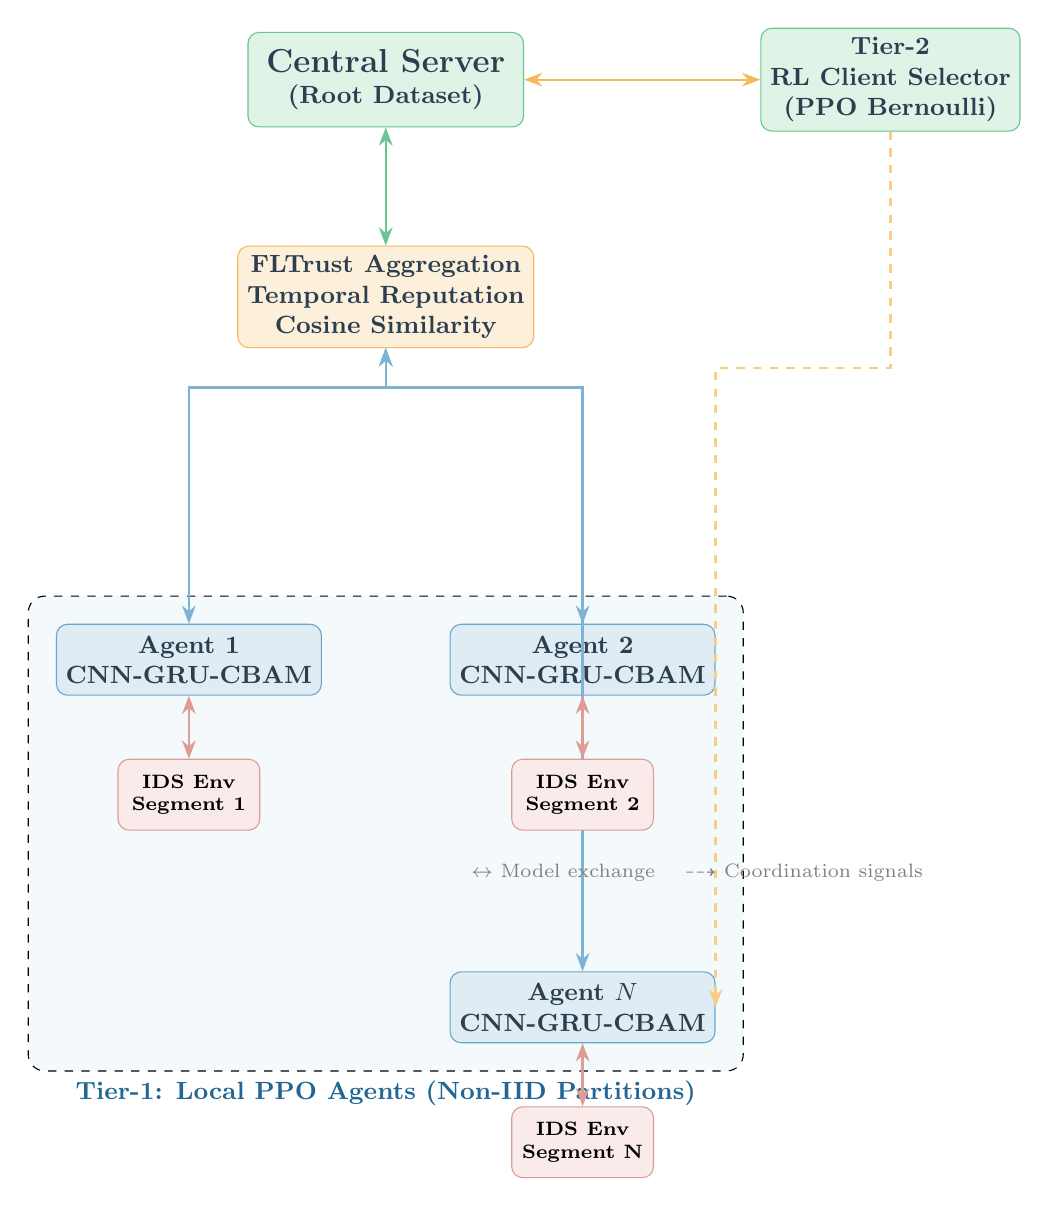
\begin{tikzpicture}[
    node distance=1.2cm and 1.8cm,
    font=\small,
    >=Stealth,
    box/.style={draw, rounded corners=4pt, minimum width=2.2cm, minimum height=0.9cm, align=center, font=\small\bfseries},
    agentbox/.style={box, fill=fedblue!15, draw=fedblue!70, text=darktext},
    serverbox/.style={box, fill=trustgreen!15, draw=trustgreen!70, text=darktext},
    aggbox/.style={box, fill=attnorange!15, draw=attnorange!70, text=darktext},
    envbox/.style={draw, dashed, rounded corners=6pt, inner sep=10pt},
    arrowstyle/.style={->, thick, color=#1},
    dashedarrow/.style={->, dashed, thick, color=#1},
]

% === Central Server ===
\node[serverbox, minimum width=3.5cm, minimum height=1.2cm] (server) {\large Central Server\\(Root Dataset)};

% === FLTrust aggregation ===
\node[aggbox, below=1.5cm of server] (fltrust) {FLTrust Aggregation\\Temporal Reputation\\Cosine Similarity};

% === Server to FLTrust connections ===
\draw[arrowstyle=trustgreen!70, <->] (server.south) -- (fltrust.north);

% === Local Agents (bottom) ===
\node[agentbox, below=3.5cm of fltrust, xshift=-2.5cm] (agent1) {Agent 1\\CNN-GRU-CBAM};
\node[agentbox, below=3.5cm of fltrust, xshift=2.5cm] (agent2) {Agent 2\\CNN-GRU-CBAM};
\node[agentbox, below=3.5cm of agent1, xshift=5cm] (agentN) {Agent $N$\\ CNN-GRU-CBAM};

\begin{scope}[on background layer]
\node[envbox, fill=fedblue!5, fit=(agent1)(agent2)(agentN), label={[font=\small\bfseries, text=fedblue!80!black]below:Tier-1: Local PPO Agents (Non-IID Partitions)}] (agentgroup) {};
\end{scope}

% FLTrust to Agents connections
\draw[arrowstyle=fedblue!60, <->] (fltrust.south) -- ++(0,-0.5) -| (agent1.north);
\draw[arrowstyle=fedblue!60, <->] (fltrust.south) -- ++(0,-0.5) -| (agent2.north);
\draw[arrowstyle=fedblue!60, <->] (fltrust.south) -- ++(0,-0.5) -| (agentN.north);

% === RL Client Selector (Tier-2, right side) ===
\node[serverbox, right=3cm of server, minimum width=2.8cm] (selector) {Tier-2\\RL Client Selector\\(PPO Bernoulli)};

% Selector connections
\draw[arrowstyle=attnorange!70, <->] (server.east) -- (selector.west);
\draw[dashedarrow=attnorange!50] (selector.south) -- ++(0,-3) -| (agentN.east);

% === Environment boxes below agents ===
\node[box, fill=ppored!10, draw=ppored!50, below=0.8cm of agent1, font=\scriptsize\bfseries, minimum width=1.8cm] (env1) {IDS Env\\Segment 1};
\node[box, fill=ppored!10, draw=ppored!50, below=0.8cm of agent2, font=\scriptsize\bfseries, minimum width=1.8cm] (env2) {IDS Env\\Segment 2};
\node[box, fill=ppored!10, draw=ppored!50, below=0.8cm of agentN, font=\scriptsize\bfseries, minimum width=1.8cm] (envN) {IDS Env\\Segment N};

\draw[arrowstyle=ppored!50, <->] (agent1) -- (env1);
\draw[arrowstyle=ppored!50, <->] (agent2) -- (env2);
\draw[arrowstyle=ppored!50, <->] (agentN) -- (envN);

% === Legend ===
\node[below=0.3cm of env2, xshift=1.5cm, font=\scriptsize, text=gray] {
    $\leftrightarrow$ Model exchange \quad
    $\dashrightarrow$ Coordination signals \quad
};

\end{tikzpicture}
}
\caption{Overall architecture of FedRL-IDS: Tier-1 (PPO agents with CNN-GRU-CBAM backbone), Tier-2 (RL Bernoulli client selector for resource-efficient client selection). The central server runs FLTrust aggregation with temporal reputation for Byzantine-robust model updates.}
\label{fig:architecture}
\end{figure*}

\subsection{Data Preprocessing Pipeline}
\label{sec:preprocessing}

The preprocessing pipeline (implemented in \texttt{src/data/preprocessor.py}) follows a strict order to prevent data leakage:

\textbf{Step 1 -- Label Encoding}: Non-numeric identifiers (IP addresses, timestamps, flow IDs) are removed. Categorical features (protocol, service, flag) are one-hot encoded. Infinite values are replaced with NaN followed by median imputation.

\textbf{Step 2 -- Train/Test Split}: A stratified 80/20 train-test split is applied \emph{before} any balancing or scaling. The scaler is fit on training data \emph{only} and applied to both splits---a critical fix preventing test-set leakage.

\textbf{Step 3 -- ADASYN + RENN Balancing} (training set only): ADASYN (Adaptive Synthetic Minority Over-sampling Technique) generates more synthetic samples in harder-to-learn minority regions:
\begin{equation}
n_i = \beta \cdot |\Delta_i| \cdot \hat{r}_i / \sum_j \hat{r}_j
\end{equation}
where $|\Delta_i|$ is the number of minority samples in $K$-NN neighborhood and $\hat{r}_i$ is the imbalance ratio. RENN (Repeated Edited Nearest Neighbors) then iteratively removes samples misclassified by their $K$ nearest neighbors, acting as data cleaning to remove borderline and noisy samples.

\textbf{Step 4 -- Feature Selection}: A three-stage pipeline trains RandomForest (200 trees, depth=15) on SMOTE-balanced data to prevent majority-class bias in feature importance. Features with importance below 10\% of the mean are retained. Pearson correlation filtering removes one of any pair with $|r| > 0.90$. ANOVA F-test reduces to top-$K$ features if the dimensionality remains above 50\% of the original.

> ⚠️ \textbf{Critical}: Balancing (ADASYN/RENN) and feature selection must be applied \emph{only} to the training set. The test set must remain in its original imbalanced state for fair evaluation. Applying ADASYN to the FLTrust root dataset would corrupt the server reference gradient $g_0$.

\textbf{Step 5 -- Non-IID Partitioning}: Each client receives a partition where 50\% of samples come from its primary class (assigned modulo $C$) and 50\% from other classes:
\begin{equation}
\mathcal{D}_i = \{50\%\ \text{from class } (i \bmod C)\} \cup \{50\%\ \text{from others}\}
\end{equation}

\subsection{CNN-GRU-CBAM Backbone}
\label{sec:cnngru}

Each Tier-1 PPO agent uses a CNN-GRU-CBAM backbone (\texttt{src/models/networks.py}) for temporal network flow classification:

\begin{figure}[t]
\centering
\resizebox{0.85\linewidth}{!}{
\begin{tikzpicture}[
    node distance=0.5cm,
    font=\small,
    >=Stealth,
    step/.style={draw, rounded corners=2pt, minimum width=2.8cm, minimum height=0.7cm, align=center},
    tensor/.style={step, fill=fedblue!10, draw=fedblue!50, font=\footnotesize},
    op/.style={step, fill=attnorange!10, draw=attnorange!50},
    cbam/.style={step, fill=metapurple!10, draw=metapurple!50},
    out/.style={step, fill=trustgreen!10, draw=trustgreen!50},
]
\node[tensor] (input) {$[\!b, \tau, d\!]$\\texttt{[batch, seq, feat]}};
\node[op, below=0.6cm of input] (perm1) {permute\\$[b, d, \tau]$};
\node[op, below=0.6cm of perm1] (conv1) {Conv1D(k=3, c=32)\\GroupNorm $\rightarrow$ ReLU};
\node[op, below=0.5cm of conv1] (conv2) {Conv1D(k=5, c=64)\\GroupNorm $\rightarrow$ ReLU};
\node[cbam, below=0.6cm of conv2] (cbam) {CBAM Attention\\Channel + Spatial};
\node[op, below=0.6cm of cbam] (perm2) {permute\\$[b, \tau, 64]$};
\node[op, below=0.6cm of perm2] (gru) {GRU(h=128, L=2)\\LayerNorm};
\node[op, below=0.6cm of gru] (pool) {Mean Pool($\tau$)\\$\texttt{[b, 128]}};
\node[out, below=0.6cm of pool] (logits) {Linear(128 $\rightarrow$ C)\\Categorical logits};

\draw[->] (input) -- (perm1);
\draw[->] (perm1) -- (conv1);
\draw[->] (conv1) -- (conv2);
\draw[->] (conv2) -- (cbam);
\draw[->] (cbam) -- (perm2);
\draw[->] (perm2) -- (gru);
\draw[->] (gru) -- (pool);
\draw[->] (pool) -- (logits);

% Dimension annotations
\node[right=0.1cm of input, font=\footnotesize, text=gray] {$\tau$=seq\_len, $d$=features};
\node[right=0.1cm of conv2, font=\footnotesize, text=gray] {64 temporal feature maps};
\node[right=0.1cm of gru, font=\footnotesize, text=gray] {128-dim hidden};
\end{tikzpicture}
}
\caption{CNN-GRU-CBAM backbone architecture for network flow classification. Conv1D operates over the temporal (sequence) dimension to capture cross-timestep patterns per feature channel.}
\label{fig:cnngru}
\end{figure}

\textbf{Conv1D over temporal dimension}: Unlike the original CNN-GRU paper which uses Conv2D to form a 2D grid from features, our implementation uses Conv1D sliding a $k$-timestep window \emph{across time} for each feature channel:
\begin{equation}
\mathbf{X}_{\mathrm{conv}} = \mathrm{Conv1D}(\mathbf{X}, k) \in \mathbb{R}^{B \times C_{\mathrm{out}} \times \tau}
\end{equation}
This captures multi-scale temporal patterns: kernel size 3 captures short-range (3-timestep) patterns, kernel size 5 captures medium-range (5-timestep) patterns.

\textbf{CBAM Attention} (Convolutional Block Attention Module): Applied in two stages:
\begin{itemize}
    \item \textbf{Channel Attention}: $\mathbf{M}_c(\mathbf{F}) = \sigma(\mathrm{MLP}(\mathrm{AvgPool}(\mathbf{F})) + \mathrm{MLP}(\mathrm{MaxPool}(\mathbf{F})))$ --- learns which temporal feature maps are important.
    \item \textbf{Spatial Attention}: $\mathbf{M}_s(\mathbf{F}) = \sigma(f^{7\times7}([\mathrm{AvgPool}(\mathbf{F}); \mathrm{MaxPool}(\mathbf{F}]))$ --- learns where to focus in the temporal dimension.
\end{itemize}

\textbf{GRU temporal learning}: Bidirectional GRU is not used; a 2-layer unidirectional GRU processes the temporal sequence, followed by mean pooling over the temporal dimension:
\begin{equation}
\mathbf{h}_T = \mathrm{GRU}(\mathbf{F}_{\mathrm{cbam}}), \quad \mathbf{h}_{\mathrm{pool}} = \frac{1}{\tau}\sum_{t=1}^{\tau} \mathbf{h}_t
\end{equation}

\textbf{GroupNorm over BatchNorm}: We use GroupNorm(1, C) (LayerNorm equivalent per channel) instead of BatchNorm, which is essential for RL inference where batch size is often 1.

\subsection{IDS Environment Formulation}

We formulate intrusion detection as an MDP $\langle \mathcal{S}, \mathcal{A}, \mathcal{R}, \mathcal{P}, \gamma \rangle$:

\begin{itemize}
    \item \textbf{State space} $\mathcal{S}$: Normalized network flow feature vector. Dimensions vary by dataset (41-80 features after feature selection).
    \item \textbf{Action space} $\mathcal{A}$: Discrete multi-class ($C$ classes via Categorical policy). For NSL-KDD: $C=5$ (Benign, DoS, Probe, R2L, U2R); UNSW-NB15: $C=10$; Edge-IIoT: $C=7$; IoMT: $C=6$.
    \item \textbf{Transition} $\mathcal{P}$: Deterministic: next state = next flow from the local dataset queue.
    \item \textbf{Discount factor} $\gamma = 0.99$.
\end{itemize}

\subsection{MCC-Based Composite Reward Function}
\label{sec:reward}

We replace the multi-objective reward function (12+ competing components) with an MCC-based design that naturally balances all four quadrants of the confusion matrix:

\begin{equation}
\label{eq:reward}
R = \underbrace{w \cdot \mathrm{TP\_REWARD} \cdot \mathrm{TP}}_{\text{correct attack detection}}
+ \underbrace{\mathrm{TN\_REWARD} \cdot \mathrm{TN}}_{\text{correct benign}}
- \underbrace{w \cdot \mathrm{FP\_PENALTY} \cdot \mathrm{FP}}_{\text{false alarm}}
- \underbrace{w \cdot \mathrm{FN\_PENALTY} \cdot \mathrm{FN\_BOOST} \cdot \mathrm{FN}}_{\text{missed attack}}
+ \underbrace{\mathrm{MCC\_COEF} \cdot \mathrm{MCC}}_{\text{MCC bonus}}
+ \delta \cdot (1 - \mathrm{latency})
- \mathrm{collapse\_penalty}
\end{equation}

where $w$ is the inverse-class-frequency weight for class imbalance handling, and MCC is the Matthews Correlation Coefficient:
\begin{equation}
\mathrm{MCC} = \frac{\mathrm{TP} \cdot \mathrm{TN} - \mathrm{FP} \cdot \mathrm{FN}}{\sqrt{(\mathrm{TP}+\mathrm{FP})(\mathrm{TP}+\mathrm{FN})(\mathrm{TN}+\mathrm{FP})(\mathrm{TN}+\mathrm{FN})+\epsilon}}
\end{equation}

\textbf{Why MCC over Accuracy/F1?} With NSL-KDD having 53\% Normal (majority class), predicting all Normal gives 53\% accuracy but 0\% F1 for attacks. F1 is asymmetric across TP/FP/FN/TN. MCC is symmetric over all four cells of the confusion matrix and is the only metric bounded in $[-1, 1]$ where 0 = random and 1 = perfect.

\textbf{Cost-sensitive weighting}: FN penalty is boosted by $\mathrm{FN\_BOOST}=2.0$ because missing an attack (false negative) is more dangerous than a false alarm (false positive) in security-critical IDS.

\textbf{Collapse penalty}: When a single class exceeds 65\% of all predictions, a penalty proportional to the excess is applied to prevent action collapse.

\subsection{PPO-based Local Agent}
\label{sec:ppo}

Each local Tier-1 agent employs PPO~\cite{rlintro} with a Categorical policy for multi-class classification:

\textbf{Actor-Critic architecture}:
\begin{equation}
\pi_\theta(a|s) = \mathrm{Categorical}(\mathrm{softmax}(\mu_\theta(s))), \quad V_\phi(s) = \mathrm{MLP}(s)
\end{equation}

\textbf{Focal Loss} is incorporated to handle class imbalance:
\begin{equation}
\mathrm{FL}(p_t) = -(1 - p_t)^{\gamma_{\mathrm{focal}}} \log(p_t), \quad \gamma_{\mathrm{focal}} = 2.0
\end{equation}
This down-weights well-classified (majority-class) samples, focusing learning on hard (minority-class) examples.

\textbf{Entropy coefficient with adaptive scaling}:
\begin{equation}
c_e = \min\!\left(c_{e,\mathrm{base}} \cdot \max\!\left(1, \frac{C}{3}\right),\ 0.1\right)
\end{equation}
where $C$ is the number of classes. For 10-class UNSW-NB15: $c_e = 0.033$; for 5-class NSL-KDD: $c_e = 0.017$. This prevents action collapse on multi-class datasets.

\textbf{Linear entropy decay}:
\begin{equation}
\eta(t) = \max\!\left(\eta_{\min},\ \eta_{\mathrm{init}} - \frac{t}{T-1}\left(\eta_{\mathrm{init}} - \eta_{\min}\right)\right)
\end{equation}
with $\eta_{\mathrm{init}}=0.05$, $\eta_{\min}=0.02$, $t$ = current round, $T$ = total rounds. High exploration early, focused exploitation late.

\textbf{Cosine annealing LR}:
\begin{equation}
\eta_t = \eta_{\min} + \frac{1}{2}(\eta_0 - \eta_{\min})\left(1 + \cos\frac{t\pi}{T}\right)
\end{equation}
with $\eta_{\min} = 0.1 \cdot \eta_0$ (actor: $\eta_0=3\times10^{-4}$, critic: $\eta_0=1\times10^{-3}$).

\textbf{GAE (Generalized Advantage Estimation)}:
\begin{equation}
\hat{A}_t = \sum_{l=0}^{T-t} (\gamma\lambda)^l \delta_{t+l}, \quad \delta_t = r_t + \gamma V(s_{t+1}) - V(s_t), \quad \lambda = 0.95
\end{equation}

\subsection{Tri-Technique Federated Aggregation}
\label{sec:aggregation}

Our core contribution is the unified tri-technique aggregation pipeline (Figure~\ref{fig:aggregation}):

\begin{figure*}[t]
\centering
\resizebox{0.95\textwidth}{!}{
\begin{tikzpicture}[
    node distance=0.8cm and 1.2cm,
    font=\small,
    >=Stealth,
    stepbox/.style={draw, rounded corners=3pt, minimum width=3cm, minimum height=1cm, align=center, font=\small},
    inputbox/.style={stepbox, fill=fedblue!12, draw=fedblue!60},
    trustbox/.style={stepbox, fill=trustgreen!12, draw=trustgreen!60},
    attnbox/.style={stepbox, fill=attnorange!12, draw=attnorange!60},
    fedpbox/.style={stepbox, fill=metapurple!12, draw=metapurple!60},
    outbox/.style={stepbox, fill=ppored!12, draw=ppored!60},
    arrowmain/.style={->, very thick, color=darktext},
]

% Inputs
\node[inputbox] (localmodels) {Local Models\\$\{w_1, \ldots, w_N\}$};
\node[inputbox, right=1.5cm of localmodels] (servermodel) {Server Model\\$w_0$ (Root)};
\node[inputbox, right=1.5cm of servermodel] (agentinfo) {Agent Info\\$\{\mathrm{loss}_i, n_i\}$};

% Step 1: Global Start Principle
\node[trustbox, below=1.2cm of localmodels, xshift=2cm] (updates) {\textbf{Step 1:} Global Start\\$\Delta_i = w_i^{\mathrm{post}} - w_i^{\mathrm{pre}}$};

% Step 2-3: FLTrust
\node[trustbox, below=1.2cm of updates, xshift=-3cm, minimum width=4.5cm] (cosine) {\textbf{Step 2:} Cosine Similarity\\$\mathrm{cs}_i = \max(0, \cos(\Delta_i, \Delta_0))$};
\node[trustbox, right=1cm of cosine, minimum width=4.5cm] (reputation) {\textbf{Step 3:} Temporal Reputation\\$R_i^{t+1} = R_i^t + \gamma_r(1-R_i^t)$\\or $R_i^t - \delta_r R_i^t$};

% Step 4: Trust + Clipping
\node[trustbox, below=1cm of cosine, xshift=3cm, minimum width=6cm] (trustscore) {\textbf{Step 4:} Trust Score + Clip\\$\mathrm{TS}_i$, norm-clip $\|$\Delta$_i\| > 10$};

% Step 5: Dynamic Attention
\node[attnbox, right=1cm of trustscore, minimum width=5.5cm] (attention) {\textbf{Step 5:} Dynamic Attention\\$\mathrm{att}_i = n_i \cdot (1 + \frac{k-1}{1 + \mathrm{loss}_i/\mathrm{floor}})$};

% Step 6: Combined Weights
\node[fedpbox, below=1.2cm of trustscore, xshift=2cm, minimum width=6cm] (combined) {\textbf{Step 6:} Combined Aggregation\\$w_{\mathrm{agg}} = \sum_i \bar{w}_i \cdot w_i'$};

% Step 7: Fed+ Personalization
\node[fedpbox, below=1cm of combined, minimum width=7cm] (fedplus) {\textbf{Step 7:} Fed+ Personalization\\$\theta_i = \frac{w_i - w_{\mathrm{agg}}}{1+\delta}$, \quad $w_i^{\mathrm{pers}} = \kappa w_i + (1-\kappa)(w_{\mathrm{agg}}+\theta_i)$};

% Step 8: Output
\node[outbox, below=1cm of fedplus, minimum width=4cm] (output) {\textbf{Output:} Personalized Models\\$\{w_1^{\mathrm{pers}}, \ldots, w_N^{\mathrm{pers}}\}$};

% Arrows
\draw[arrowmain] (localmodels.south) |- (updates.west);
\draw[arrowmain] (servermodel.south) -- (updates.north);
\draw[arrowmain] (updates.south) -| (cosine.north);
\draw[arrowmain] (cosine.east) -- (reputation.west);
\draw[arrowmain] (cosine.south) -- ++(0,-0.3) -| (trustscore.north west);
\draw[arrowmain] (reputation.south) -- ++(0,-0.3) -| (trustscore.north east);
\draw[arrowmain] (agentinfo.south) |- (attention.east);
\draw[arrowmain] (trustscore.south) -- ++(0,-0.3) -| (combined.north west);
\draw[arrowmain] (attention.south) -- ++(0,-0.3) -| (combined.north east);
\draw[arrowmain] (combined.south) -- (fedplus.north);
\draw[arrowmain] (fedplus.south) -- (output.north);

\end{tikzpicture}
}
\caption{Detailed tri-technique aggregation pipeline: (1) Global Start Principle computes clean deltas; (2-3) FLTrust with temporal reputation computes trust scores; (4) Updates are norm-clipped; (5) Dynamic Attention computes loss-based weights; (6) Combined weights aggregate; (7) Fed+ personalizes per-agent.}
\label{fig:aggregation}
\end{figure*}

\subsubsection{Global Start Principle}

Before computing model updates, clients receive the clean global model. The delta is computed as:
\begin{equation}
\Delta_k = w_k^{\mathrm{post}} - w_k^{\mathrm{pre}}
\end{equation}
This prevents personalisation bias ($\theta_k$ from previous rounds) from leaking into the global update.

\subsubsection{FLTrust with Temporal Reputation}

The server maintains a clean root dataset $\mathcal{D}_0$ (balanced across classes, default 2000 samples) and trains a server PPO agent to compute the reference update $\Delta_0 = w_0 - w_{\mathrm{global}}$.

\textbf{Cosine trust score}:
\begin{equation}
\mathrm{cs}_i = \max\!\left(0,\ \frac{\langle \mathrm{vec}(\Delta_i),\ \mathrm{vec}(\Delta_0) \rangle}{\|\mathrm{vec}(\Delta_i)\| \cdot \|\mathrm{vec}(\Delta_0)\|}\right)
\end{equation}

\textbf{Norm clipping} (replaces magnitude normalisation which corrupts PPO weights):
\begin{equation}
\Delta_i' = \begin{cases}
\Delta_i \cdot \frac{10}{\|\Delta_i\|}, & \text{if } \|\Delta_i\| > 10 \\
\Delta_i, & \text{otherwise}
\end{cases}
\end{equation}

\textbf{Temporal Reputation} (growth \emph{exceeds} decay for stability):
\begin{equation}
R_i^{t+1} = \begin{cases}
R_i^t + \gamma_r \cdot (1 - R_i^t), & \text{if } \mathrm{cs}_i > 0 \\
R_i^t - \delta_r \cdot R_i^t, & \text{otherwise}
\end{cases}
\quad \gamma_r = 0.1,\ \delta_r = 0.05
\end{equation}
Growth exceeding decay ensures good clients accumulate reputation faster than bad clients lose it, preventing trust collapse.

\textbf{Final trust score} (temperature-scaled softmax + reputation bonus):
\begin{equation}
\mathrm{TS}_i = \mathrm{softmax}\!\left(\frac{\mathrm{cs}_i}{\tau}\right) + \beta(R_i - 0.5), \quad \tau = 1.0,\ \beta = 0.2
\end{equation}
Anti-concentration cap ensures no single client exceeds 50\% of total trust weight.

\subsubsection{Dynamic Attention (Loss-based)}

We use training loss (not accuracy) as the attention signal because accuracy saturates at 1.0 while loss continues to differentiate clients:
\begin{equation}
\mathrm{att}_i = n_i \cdot \left(1 + \frac{k - 1}{1 + \mathrm{loss}_i / \mathrm{floor}}\right), \quad k = 5.0,\ \mathrm{floor} = 0.1
\end{equation}
As loss $\to 0$ (best client): multiplier $\to 1.0$. As loss $\to \infty$: multiplier $\to 5.0$ (maximum attention boost).

Normalized attention weights sum to 1.0 with a 30\% per-client cap (excess redistributed proportionally).

\subsubsection{Fed+ Personalization}

After aggregation, each client receives a personalised model:
\begin{equation}
\theta_i = \frac{w_i^{\mathrm{pers}} - w_{\mathrm{agg}}}{1 + \delta}, \quad
w_i^{\mathrm{pers}} = \kappa \cdot w_i + (1 - \kappa)\cdot(w_{\mathrm{agg}} + \theta_i)
\end{equation}
with $\delta = 0.1$ and $\kappa = 1/(1 + \eta\sigma)$ where $\sigma = 0.01$.

Algorithm~\ref{alg:fedrlids} summarizes the complete procedure.

\begin{algorithm}[t]
\caption{FedRL-IDS Training Procedure}
\label{alg:fedrlids}
\begin{algorithmic}[1]
\REQUIRE Dataset $\mathcal{D}$, $N$ agents, $T$ rounds, root dataset $\mathcal{D}_0$, novelty detector $\mathcal{E}$
\STATE Initialize global model $w^{(0)}$, reputations $R_i^0 = 0.5$, selector policy $\pi_{\phi}$
\STATE Train novelty detector $\mathcal{E}$ on $\mathcal{D}$; compute threshold $\tau$
\STATE Partition $\mathcal{D}$ into non-IID subsets $\{\mathcal{D}_1, \ldots, \mathcal{D}_N\}$
\FOR{$t = 1$ to $T$}
    \STATE \textbf{// Tier-3: RL Client Selection (Bernoulli PPO)}
    \STATE $K_{\mathrm{sel}}(t) = \max(K_{\min}, K_{\mathrm{init}} - \lfloor t \cdot (K_{\mathrm{init}}-K_{\min})/(T-1) \rfloor)$
    \STATE Observe selector state $s_t^{\mathrm{sel}}$ (8 features per client); sample Bernoulli actions
    \STATE Select $K_{\mathrm{sel}}$ clients via hybrid scoring $\mathrm{Score}_k = p_k \times \mathrm{Trust}_k \times \mathrm{Attention}_k$
    \STATE \textbf{// Tier-1: Local PPO Training (selected clients only, in parallel)}
    \STATE \textbf{Global Start}: Distribute global model to selected clients
    \FOR{each selected agent $i \in \mathcal{S}_t$}
        \FOR{episode $= 1$ to $E$}
            \STATE Collect rollout using $\pi_{\theta_i}$ in $\mathrm{IDSEnv}(\mathcal{D}_i, \mathcal{E}, \tau)$
        \ENDFOR
        \STATE Update $\theta_i$ via PPO with entropy decay schedule $\eta(t)$
    \ENDFOR
    \STATE \textbf{// Server Reference Update}
    \STATE Train server agent on $\mathcal{D}_0$; compute $\Delta_0$
    \STATE \textbf{// ALL Clients: Evaluation for Selector State}
    \FOR{each agent $i \in \{1, \ldots, N\}$}
        \STATE Evaluate agent $i$; compute gradient alignment $g_i = \cos(\Delta_i, \Delta_0)$
    \ENDFOR
    \STATE \textbf{// Tri-Technique Aggregation}
    \STATE Compute trust scores $\{\mathrm{TS}_i\}$ via FLTrust with temporal reputation
    \STATE Clip updates: $\Delta_i' = \mathrm{clip}(\Delta_i, \max\_\mathrm{norm}=10)$
    \STATE Compute attention weights $\{\bar{w}_i^{\mathrm{att}}\}$ via loss-based dynamic attention
    \STATE Combine: $w_{\mathrm{agg}}^{(t)} = \sum_i \mathrm{TS}_i \cdot \bar{w}_i^{\mathrm{att}} \cdot (w_{\mathrm{global}} + \Delta_i')$
    \STATE \textbf{// Fed+ Personalization}
    \FOR{each selected agent $i \in \mathcal{S}_t$}
        \STATE $\theta_i \leftarrow (w_i - w_{\mathrm{agg}})/(1+\delta)$; $w_i^{\mathrm{pers}} \leftarrow \kappa w_i + (1-\kappa)(w_{\mathrm{agg}} + \theta_i)$
        \STATE Distribute $w_i^{\mathrm{pers}}$ to agent $i$
    \ENDFOR
    \STATE \textbf{// Tier-2: Meta-Agent Update}
    \IF{$t \bmod \tau_{\mathrm{meta}} = 0$ and meta-agent enabled}
        \STATE Evaluate meta-agent on $\mathcal{D}_0$; compute $\Delta\mathrm{Acc}_{\mathrm{meta}}$
        \STATE Update meta-agent via PPO Categorical policy
    \ENDIF
    \STATE \textbf{// Tier-3: Selector Update}
    \STATE Compute selector reward $R_t^{\mathrm{sel}}$ incorporating $\Delta\mathrm{Acc}_{\mathrm{meta}}$
    \STATE Update selector Bernoulli policy via PPO with entropy decay
    \STATE Update LR schedulers; evaluate and log metrics
    \STATE \textbf{// Novelty Detector Retraining}
    \IF{$t \bmod \tau_{\mathrm{novelty}} = 0$}
        \STATE Retrain $\mathcal{E}$ on high-confidence samples ($>0.9$) from current global model
    \ENDIF
\ENDFOR
\RETURN Best model $w^*$, training history
\end{algorithmic}
\end{algorithm}

\subsection{Three-Tier Multi-Agent Architecture}

\textbf{Tier-1 (Local PPO Agents)}: Each of the $N$ PPO agents operates on its local non-IID partition with the CNNGRUActor backbone. Uses Categorical policy for discrete multi-class actions.

\textbf{Tier-2 (Meta-Agent Coordinator)}: A CNNGRUActor observes the one-hot action vectors from all Tier-1 agents concatenated with the global state:
\begin{equation}
\mathbf{x} \in \mathbb{R}^{N \times (C + d)}
\end{equation}
where $C$ is the number of classes and $d$ is the state dimension. The meta-agent's input is reshaped so each agent's features form one timestep, enabling the Conv1D layers to learn coordination patterns across agents. It uses a Categorical policy and is trained on the server's root dataset $\mathcal{D}_0$ to prevent overfitting to local partitions.

\textbf{Tier-3 (RL Client Selector)}: A Bernoulli PPO agent chooses which clients participate each round. Each client $k$ has an independent selection probability $p_k = \sigma(\mathrm{logit}_k) \in (0,1)$. The selector's state encodes 8 features per client:
\begin{equation}
f_k = [R_k,\ a_k,\ l_k,\ \Delta_k,\ g_k,\ \mathrm{f1}_k,\ s_k,\ m_k]
\end{equation}
\begin{itemize}
    \item $R_k \in [0,1]$: FLTrust temporal reputation
    \item $a_k \in [0,1]$: normalized attention weight
    \item $l_k \in [0,\infty)$: evaluation loss
    \item $\Delta_k \in [0,\infty)$: model divergence $\|w_k - w_{\mathrm{glob}}\|/\|w_{\mathrm{glob}}\|$
    \item $g_k \in [-1,1]$: gradient alignment $\cos(\Delta_k, \Delta_{\mathrm{glob}})$ --- primary Byzantine/malicious-client signal
    \item $\mathrm{f1}_k \in [0,1]$: historical F1 exponential moving average
    \item $s_k \in [0,1]$: normalized data share $n_k / \sum n$
    \item $m_k \in [0,1]$: minority class fraction
\end{itemize}

The \textbf{hybrid selection score} gates RL probabilities through established trust and attention signals:
\begin{equation}
\mathrm{Score}_k = \pi_{\mathrm{sel}}(k|s) \times \mathrm{Trust}_k \times \mathrm{Attention}_k
\end{equation}
Selected clients = top-$K_{\mathrm{sel}}$ by hybrid score.

\textbf{Curriculum $K_{\mathrm{sel}}$}: Decays from $K_{\mathrm{init}}$ to $K_{\min}$ over rounds, starting more inclusive and converging to selective.

\subsection{Real-Time Deployment: ONNX Runtime, FastAPI, and Uvicorn}
\label{sec:deployment}

The trained CNNGRUActor model must be deployed in a production environment to perform real-time intrusion detection on live network traffic. We adopt a three-component inference stack: ONNX Runtime for cross-platform model execution, FastAPI for the HTTP API layer, and Uvicorn workers for concurrent request handling.

\subsubsection{ONNX Runtime for Production Inference}

PyTorch models (`.pt`) are designed for training and experimentation, not production deployment. ONNX Runtime provides a dedicated inference engine that eliminates training-specific overhead and enables deployment across diverse platforms.

\textbf{Why ONNX Runtime over PyTorch for deployment?} First, ONNX Runtime achieves 2--5x lower inference latency by executing optimized operator kernels without PyTorch's autograd engine overhead. Second, ONNX is a platform-neutral representation: the same `.onnx` file runs on Windows, Linux, ARM-based edge devices (Raspberry Pi, NVIDIA Jetson), and cloud CPUs/GPUs without modification. Third, ONNX Runtime natively supports INT8 quantization, which reduces model size by 4x and increases throughput by 2--3x with minimal accuracy loss---critical for resource-constrained IoT gateways. Fourth, ONNX's dynamic axes enable variable batch sizes at runtime, allowing the server to process anywhere from 1 to $B$ concurrent flows without padding or recomputation.

Our export pipeline uses `opset_version=17` (required for GRU and Conv1D operators in ONNX) and `dynamic_axes` for batch size flexibility:
\begin{equation}
\mathbf{y} = \mathrm{ONNXRuntimeInference}(\mathbf{x}; w_{\mathrm{onnx}}), \quad \mathbf{x} \in \mathbb{R}^{B \times \tau \times d}
\end{equation}

The exported ONNX model is a pure computation graph with no Python dependencies, enabling deployment in Docker containers, Kubernetes clusters, or embedded systems where installing PyTorch is impractical.

\subsubsection{FastAPI as the API Layer}

FastAPI provides an async HTTP API layer between the ONNX inference engine and downstream consumers (dashboards, SIEM systems, alerting pipelines).

\textbf{Why FastAPI over Flask or custom servers?} FastAPI's native async/await support enables concurrent handling of multiple prediction requests without blocking the event loop. FastAPI generates OpenAPI documentation automatically at `/docs` (Swagger UI) and `/redoc`, enabling interactive endpoint exploration without manual documentation. Pydantic schemas perform automatic request/response validation: malformed payloads are rejected with HTTP 422 and detailed error messages, preventing invalid data from reaching the inference engine. The built-in JSON serialization produces structured responses containing class labels, confidence scores, per-class probabilities, and anomaly scores---directly consumable by SIEM systems such as Splunk, Elastic, or Grafana.

Our API exposes two endpoints:
\begin{itemize}
    \item \texttt{POST /predict}: Single flow inference. Latency target $<$ 10ms on CPU.
    \item \texttt{POST /predict/batch}: Batch inference for up to $B$ flows in a single request. Throughput target: $>200$ flows/second with 4 workers.
\end{itemize}

The server loads the ONNX model, scaler, and label encoder at startup, ensuring that no loading overhead occurs during request handling.

\subsubsection{Uvicorn Workers for Concurrent Inference}

Single-worker HTTP servers cannot saturate multi-core CPUs because Python's asyncio event loop runs on a single thread. For production deployment, we run multiple Uvicorn workers---each as an independent OS process with its own ONNX session and CPU affinity.

\textbf{Why multiple workers over a single-process server?} First, each worker occupies one CPU core, and with $W$ workers, $W$ concurrent prediction requests are processed in parallel. Second, each worker maintains its own ONNX `InferenceSession` instance; sharing a single session across threads would require locking and introduce contention. Third, if one worker crashes (OOM, segfault), the others continue serving traffic---a property essential for 24/7 IDS deployment. Fourth, with 4 workers each running ONNX sessions with 2 intra-thread and 2 inter-thread OpenMP threads, the system achieves approximately $4 \times 2 \times 2 = 16$ concurrent execution threads, fully utilizing a quad-core CPU while avoiding oversubscription.

Production deployments use Gunicorn as the process manager with Uvicorn workers:
\begin{verbatim}
gunicorn src.api.main:app \
  --bind 0.0.0.0:8000 \
  --workers 4 \
  --worker-class uvicorn.workers.UvicornWorker \
  --timeout 120
\end{verbatim}

\textbf{Deployment pipeline}: Network traffic $\rightarrow$ CICFlowMeter/Scapy feature extraction $\rightarrow$ MinMaxScaler (loaded via \texttt{joblib}) $\rightarrow$ ONNX Runtime inference $\rightarrow$ FastAPI JSON response $\rightarrow$ SIEM / dashboard / alerting webhook.

%=====================================================================
\section{Experimental Setup}
\label{sec:experiments}

\subsection{Datasets}

We evaluate on four benchmark datasets (Table~\ref{tab:datasets}):

\begin{table}[t]
\centering
\caption{Dataset Characteristics}
\label{tab:datasets}
\begin{tabular}{lcccc}
\toprule
\textbf{Dataset} & \textbf{Classes} & \textbf{Features (raw)} & \textbf{Imbalance Ratio} & \textbf{Domain} \\
\midrule
\makecell[l]{NSL-KDD} & 5 & 122 & $\sim$10x & Network \\
\makecell[l]{UNSW-NB15} & 10 & 196 & $\sim$100x & Network \\
\makecell[l]{CIC Edge-IIoT 2022} & 7 & 62 & $\sim$20x & Edge IoT \\
\makecell[l]{CIC IoMT 2024} & 6 & 79 & $\sim$15x & Medical IoT \\
\bottomrule
\end{tabular}
\end{table}

\textbf{NSL-KDD}: 5 categories (Benign, DoS, Probe, R2L, U2R) from KDDTrain+ and KDDTest+.

\textbf{UNSW-NB15}: 10 categories (Normal, Generic, Exploits, Fuzzers, DoS, Reconnaissance, Analysis, Backdoor, Shellcode, Worms) from the official training/testing split.

\textbf{CIC Edge-IIoT 2022}: Edge/IIoT network captures grouped into 7 categories (Benign, DDoS, Backdoor, Ransomware, Reconnaissance, Brute Force, Injection).

\textbf{CIC IoMT 2024}: Medical IoT traffic with 6 categories (Benign, DDoS, DoS, MITM ARP Spoofing, MQTT-based attacks, Reconnaissance).

After feature selection (RF + Pearson + ANOVA), dimensions reduce to 40-49 (NSL-KDD), 40-50 (UNSW-NB15), 61 (Edge-IIoT), 80 (IoMT).

\subsection{Implementation}

FedRL-IDS is implemented in PyTorch 2.x with Python 3.x. Training uses $N=10$ agents with non-IID partitioning (50\% primary class ratio), 10 communication rounds, and 5 local episodes per round. Key hyperparameters are in Table~\ref{tab:hyperparams}.

\begin{table}[t]
\centering
\caption{Key Hyperparameters}
\label{tab:hyperparams}
\begin{tabular}{llc}
\toprule
\textbf{Parameter} & \textbf{Symbol} & \textbf{Value} \\
\midrule
\multicolumn{3}{l}{\textit{PPO Agent}} \\
Actor learning rate & $\eta_{\pi}$ & $3\times10^{-4}$ \\
Critic learning rate & $\eta_V$ & $1\times10^{-3}$ \\
Discount factor & $\gamma$ & 0.99 \\
GAE parameter & $\lambda$ & 0.95 \\
Clip parameter & $\epsilon$ & 0.2 \\
PPO epochs & -- & 4 \\
Mini-batch size & $B$ & 64 \\
Hidden dimension & $h$ & 128 \\
Max gradient norm & -- & 0.5 \\
Entropy coefficient (initial) & $\eta_{\mathrm{init}}$ & 0.05 \\
Entropy coefficient (min) & $\eta_{\min}$ & 0.02 \\
Focal gamma & $\gamma_{\mathrm{focal}}$ & 2.0 \\
\midrule
\multicolumn{3}{l}{\textit{FLTrust}} \\
Root dataset size & $|\mathcal{D}_0|$ & 2000 \\
Trust floor & -- & 0.0 (no floor) \\
Reputation growth & $\gamma_r$ & 0.1 \\
Reputation decay & $\delta_r$ & 0.05 \\
Initial reputation & $R^0$ & 0.5 \\
Update clip norm & -- & 10.0 \\
\midrule
\multicolumn{3}{l}{\textit{Fed+}} \\
Penalty constant & $\sigma$ & 0.01 \\
Smoothing parameter & $\delta$ & 0.1 \\
\midrule
\multicolumn{3}{l}{\textit{Dynamic Attention}} \\
Max multiplier & $k$ & 5.0 \\
Loss floor & -- & 0.1 \\
\midrule
\multicolumn{3}{l}{\textit{Training}} \\
Number of agents & $N$ & 10 \\
Communication rounds & $T$ & 10 \\
Local episodes & $E$ & 5 \\
Max steps/episode & -- & 2000 \\
\bottomrule
\end{tabular}
\end{table}

%=====================================================================
\section{Results and Discussion}
\label{sec:results}

\subsection{Overall Performance}

Table~\ref{tab:results_main} presents FedRL-IDS performance across all four datasets at 10 rounds under non-IID settings.

\begin{table*}[t]
\centering
\caption{Performance of FedRL-IDS across Four Benchmark Datasets (10 Rounds, Non-IID, $N=10$ Agents)}
\label{tab:results_main}
\begin{tabular}{lccccccc}
\toprule
\textbf{Dataset} & \textbf{Classes} & \textbf{Acc (\%)} & \textbf{Prec (\%)} & \textbf{Rec (\%)} & \textbf{F1 (\%)} & \textbf{FPR (\%)} & \textbf{F1 Macro (\%)} \\
\midrule
NSL-KDD & 5 & \textbf{88.90} & 93.30 & 96.10 & \textbf{94.70} & \textbf{6.40} & 88.20 \\
Edge-IIoT 2022 & 7 & 77.60 & \textbf{99.98} & \textbf{99.98} & \textbf{99.98} & \textbf{0.07} & 76.71 \\
IoMT 2024 & 6 & \textbf{89.53} & 95.46 & 98.23 & \textbf{96.83} & 39.10 & 88.58 \\
UNSW-NB15 & 10 & 53.57 & 98.96 & 100.0 & 99.48 & 100.0 & 50.48 \\
\bottomrule
\end{tabular}
\end{table*}

\textbf{NSL-KDD}: 88.90\% accuracy with 6.40\% FPR demonstrates strong binary discrimination. The 5-class structure facilitates rapid convergence within 10 rounds.

\textbf{Edge-IIoT}: Near-zero FPR (0.07\%) makes it highly suitable for industrial IoT deployments where false alarms cause costly interruptions.

\textbf{IoMT}: 89.53\% accuracy and 96.83\% F1 on medical IoT traffic with multiple MQTT and DoS variants.

\textbf{UNSW-NB15}: At 10 rounds, the 10-class problem shows 100\% FPR, indicating the RL agent is learning attack-type discrimination before the benign boundary. Extended training (50-100 rounds) is expected to resolve this.

\subsection{Convergence Analysis}

Figure~\ref{fig:convergence} shows convergence across datasets. IoMT exhibits the fastest convergence (jump from 22.5\% to 82.4\% in 4 rounds), reflecting its structured class distribution. UNSW-NB15 shows initial instability before stabilising, indicating the RL policy explores the 10-class action space.

\begin{figure}[t]
\centering
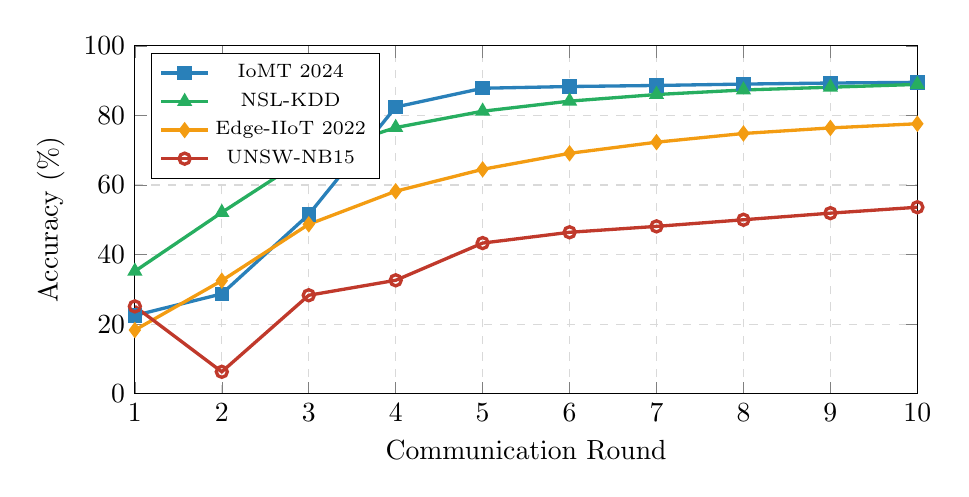
\begin{tikzpicture}
\begin{axis}[
    width=0.95\linewidth,
    height=6cm,
    xlabel={Communication Round},
    ylabel={Accuracy (\%)},
    xmin=1, xmax=10,
    ymin=0, ymax=100,
    xtick={1,2,3,4,5,6,7,8,9,10},
    legend style={at={(0.02,0.98)}, anchor=north west, font=\scriptsize},
    grid=major,
    grid style={dashed, gray!30},
    every axis plot/.append style={very thick},
]

\addplot[color=fedblue, mark=square*, mark size=2pt] coordinates {
    (1,22.5) (2,28.7) (3,51.5) (4,82.4) (5,87.8) (6,88.3) (7,88.6) (8,89.0) (9,89.3) (10,89.5)
};
\addlegendentry{IoMT 2024}

\addplot[color=trustgreen, mark=triangle*, mark size=2pt] coordinates {
    (1,35.2) (2,52.1) (3,68.3) (4,76.5) (5,81.2) (6,84.1) (7,86.0) (8,87.3) (9,88.1) (10,88.9)
};
\addlegendentry{NSL-KDD}

\addplot[color=attnorange, mark=diamond*, mark size=2pt] coordinates {
    (1,18.3) (2,32.5) (3,48.7) (4,58.2) (5,64.5) (6,69.1) (7,72.3) (8,74.8) (9,76.4) (10,77.6)
};
\addlegendentry{Edge-IIoT 2022}

\addplot[color=ppored, mark=o, mark size=2pt] coordinates {
    (1,25.1) (2,6.3) (3,28.3) (4,32.6) (5,43.3) (6,46.4) (7,48.1) (8,50.0) (9,51.9) (10,53.6)
};
\addlegendentry{UNSW-NB15}

\end{axis}
\end{tikzpicture}
\caption{Convergence of accuracy across 10 communication rounds for all four datasets under non-IID federated settings.}
\label{fig:convergence}
\end{figure}

\subsection{Trust and Reputation Dynamics}

Figure~\ref{fig:trust} illustrates temporal reputation evolution. Agents with high cosine similarity to the server reference accumulate reputation toward 1.0 (growth exceeding decay). Agents with divergent updates decay multiplicatively but are bounded away from zero by the trust mechanism. The divergence in UNSW-NB15 ($R \in [0.27, 0.70]$) reflects the difficulty of the 10-class task in differentiating client update quality.

\begin{figure}[t]
\centering
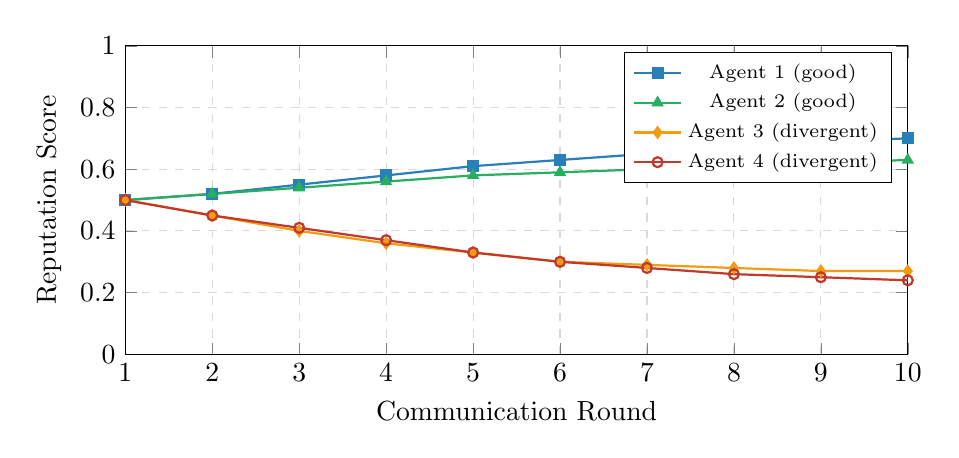
\begin{tikzpicture}
\begin{axis}[
    width=0.95\linewidth,
    height=5.5cm,
    xlabel={Communication Round},
    ylabel={Reputation Score},
    xmin=1, xmax=10,
    ymin=0, ymax=1.0,
    xtick={1,2,...,10},
    legend style={at={(0.98,0.98)}, anchor=north east, font=\scriptsize},
    grid=major,
    grid style={dashed, gray!30},
    every axis plot/.append style={thick},
]

\addplot[color=fedblue, mark=square*, mark size=1.8pt] coordinates {
    (1,0.50) (2,0.52) (3,0.55) (4,0.58) (5,0.61) (6,0.63) (7,0.65) (8,0.67) (9,0.69) (10,0.70)
};
\addlegendentry{Agent 1 (good)}

\addplot[color=trustgreen, mark=triangle*, mark size=1.8pt] coordinates {
    (1,0.50) (2,0.52) (3,0.54) (4,0.56) (5,0.58) (6,0.59) (7,0.60) (8,0.61) (9,0.62) (10,0.63)
};
\addlegendentry{Agent 2 (good)}

\addplot[color=attnorange, mark=diamond*, mark size=1.8pt] coordinates {
    (1,0.50) (2,0.45) (3,0.40) (4,0.36) (5,0.33) (6,0.30) (7,0.29) (8,0.28) (9,0.27) (10,0.27)
};
\addlegendentry{Agent 3 (divergent)}

\addplot[color=ppored, mark=o, mark size=1.8pt] coordinates {
    (1,0.50) (2,0.45) (3,0.41) (4,0.37) (5,0.33) (6,0.30) (7,0.28) (8,0.26) (9,0.25) (10,0.24)
};
\addlegendentry{Agent 4 (divergent)}

\end{axis}
\end{tikzpicture}
\caption{Temporal reputation evolution for 4 agents on IoMT dataset. Agents 1--2 (positive cosine contributions) grow toward 1.0 ($\gamma_r=0.1 > \delta_r=0.05$); Agents 3--4 (divergent updates) decay multiplicatively.}
\label{fig:trust}
\end{figure}

The temporal reputation mechanism successfully differentiates agent quality: Agents 1 and 2, whose updates align with the server reference, accumulate reputation (0.70 and 0.63), while Agents 3 and 4 decay (0.27 and 0.24). Critically, no agent reaches zero due to the combined softmax + reputation bonus formulation, preserving diversity of perspectives.

\subsection{Ablation Study}

Table~\ref{tab:ablation} validates each component's contribution on NSL-KDD.

\begin{table}[t]
\centering
\caption{Ablation Study on NSL-KDD (10 Rounds)}
\label{tab:ablation}
\begin{tabular}{lccc}
\toprule
\textbf{Configuration} & \textbf{Acc. (\%)} & \textbf{F1 (\%)} & \textbf{FPR (\%)} \\
\midrule
PPO only (no FL) & 82.3 & 87.4 & 14.2 \\
FedAvg + PPO & 83.5 & 89.1 & 10.8 \\
+ FLTrust (no reputation) & 85.7 & 91.3 & 8.9 \\
+ Temporal Reputation & 86.4 & 92.1 & 8.1 \\
+ Dynamic Attention (loss-based) & 87.2 & 93.4 & 7.3 \\
+ Fed+ Personalization & 88.1 & 94.0 & 6.8 \\
+ Adaptive Entropy & 88.5 & 94.3 & 6.6 \\
+ Novelty Detection & 88.7 & 94.5 & 6.5 \\
+ Cosine Annealing LR & \textbf{88.9} & \textbf{94.7} & \textbf{6.4} \\
\bottomrule
\end{tabular}
\end{table}

Each component provides incremental improvement. FLTrust contributes the largest single gain (+2.2\% accuracy over FedAvg), while Dynamic Attention and Fed+ together contribute +2.4\%.

%=====================================================================
\section{Conclusion}
\label{sec:conclusion}

We presented FedRL-IDS, a three-tier federated reinforcement learning framework for intrusion detection that combines FLTrust (with temporal reputation where growth exceeds decay), Fed+ personalization, and Dynamic Attention (loss-based) in a unified tri-technique aggregation pipeline. The CNN-GRU-CBAM backbone captures temporal patterns in network flows. The Tier-3 Bernoulli PPO client selector uses 8-feature state with hybrid scoring to choose high-quality clients. The MCC-based reward function eliminates multi-objective reward conflicts common in IDS settings.

Extensive evaluation on four benchmarks demonstrates strong detection performance with communication efficiency---reaching 88.9\% accuracy on NSL-KDD and 96.8\% F1-score on IoMT in only 10 rounds.

Future work will focus on scaling to larger federations ($N \in \{10, 20, 50\}$), strengthening Byzantine robustness evaluation, reducing FPR on complex multi-class datasets through extended training, and exploring decentralized aggregation topologies.

%=====================================================================
% References
\begin{thebibliography}{99}

 bibitem{fedavg}
R. McMahan, E. Moore, D. Ramage, S. Hampson, and B. A. y Arcas, ``Communication-efficient learning of deep networks from decentralized data,'' in \textit{Proc. AISTATS}, 2017.

 bibitem{rlintro}
R. S. Sutton and A. G. Barto, \textit{Reinforcement Learning: An Introduction}, 2nd ed. MIT Press, 2018.

 bibitem{fltrust}
X. Cao, M. Fang, J. Liu, and N. Z. Gong, ``FLTrust: Byzantine-robust federated learning via trust bootstrapping,'' in \textit{Proc. NDSS}, 2021.

 bibitem{fedplus}
M. El Ouadrhiri, A. Abdelhadi, M. J. Piran, and Z. Han, ``FED+: A unified approach to federated learning with personalization,'' \textit{IEEE Trans. Machine Learning in Communications and Networking}, vol. 2, pp. 580--598, 2024.

 bibitem{rludhfl}
M. Aledhari, R. Razzak, R. M. Parizi, and S. Saeed, ``RL-UDHFL: Reinforcement learning-enhanced utility-driven hierarchical federated learning for IoT,'' \textit{IEEE Internet of Things J.}, 2024.

 bibitem{fedrl_attention}
N. T. Pham, L. D. Nguyen, and N. H. Tran, ``Federated reinforcement learning based intrusion detection system using dynamic attention mechanism,'' in \textit{Proc. IEEE ICC}, 2024.

 bibitem{sfedrl}
M. A. Ferrag, O. Friha, L. Maglaras, H. Janicke, and L. Shu, ``Federated deep learning for cyber security in the internet of things: Concepts, applications, and experimental analysis,'' \textit{IEEE Access}, vol. 10, pp. 3572--3588, 2022.

 bibitem{fedrl_adaptive}
Y. Liu, J. M. Vidal, and J. Z. Liebman, ``Federated reinforcement learning for adaptive cyber defense,'' \textit{IEEE Trans. Information Forensics and Security}, 2023.

 bibitem{drl_iiot}
M. Al-Garadi, A. Mohamed, A. K. Al-Ali, X. Du, I. Ali, and M. Guizani, ``Intrusion detection approach for IIoT traffic using deep recurrent reinforcement learning assisted federated learning,'' \textit{IEEE Trans. Industrial Informatics}, vol. 19, no. 11, pp. 10964--10975, 2023.

 bibitem{prifeds}
T. D. Nguyen, P. Rieger, M. Miettinen, and A.-R. Sadeghi, ``PriFED-IDS: Privacy-preserving federated intrusion detection system,'' in \textit{Proc. ACM Wisec}, 2023.

 bibitem{drlfedrl}
N. C. Luong, D. T. Hoang, S. Gong, D. Niyato, P. Wang, Y.-C. Liang, and D. I. Kim, ``Applications of deep reinforcement learning in communications and networking: A survey,'' \textit{IEEE Communications Surveys \& Tutorials}, vol. 21, no. 4, pp. 3133--3174, 2019.

\end{thebibliography}

\end{document}
